\documentclass{deimj}
\usepackage[dvipdfmx]{graphicx}
\usepackage[ipaex]{pxchfon}
\usepackage[hyphens]{url}
\usepackage{tabularx}
\usepackage{multirow}
\usepackage{otf}

% 印刷位置調整 %
% 必要に応じて値を変更してください.
\hoffset -10mm % <-- 左に 10mm 移動
\voffset -10mm % <-- 上に 10mm 移動

\newcommand{\AmSLaTeX}{%
$\mathcal A$\lower.4ex\hbox{$\!\mathcal M\!$}$\mathcal S$-\LaTeX}
\newcommand{\PS}{{\scshape Post\-Script}}
\def\BibTeX{{\rmfamily B\kern-.05em{\scshape i\kern-.025em b}\kern-.08em
T\kern-.1667em\lower.7ex\hbox{E}\kern-.125em X}} 

% \papernumber{DEIM Forum 2019 H7-2}

\jtitle{地図上における未訪問スポットの説明性向上のための\\観光スポットの対応関係可視化手法}
%\jsubtitle{サブタイトル} <- サブタイトルを付けたいときはこの行の先頭の % を取る
\authorlist{%
 \authorentry[em18011@ns.kogakuin.ac.jp]{潘 健太}{KENTA HAN}{Univ}
 \authorentry[kitayama@cc.kogakuin.ac.jp]{北山 大輔}{DAISUGE KITAYAMA}{Univ}
 }

\affiliate[Univ]{工学院大学大学院工学研究科情報学専攻\hskip1zw
  〒163--8677 東京都新宿区西新宿1--24--2}
 {School of Engineering,Kogakuin University\\
  1--24--2,Nisisinjyuku,Tokyo,163--8677 Japan}
% \affiliate[UnivN]{工学院大学情報学部システム数理学科\hskip1zw
%   〒163--8677 東京都新宿区西新宿1--24--2}
%  {School of Engineering,Kogakuin University\\
%   1--24--2,Nisisinjyuku,Tokyo,163--8677 Japan}

\begin{document}
\pagestyle{empty}
\begin{jabstract}
近年,ユーザはWeb上の観光情報を活用して旅行計画を立てることが多くなっている.
しかし,旅行は一般的に訪れたことがないスポットに行くことが多いため,観光情報を適切に理解することは困難である.
そこで,訪問したことがある観光スポットの特徴を用いて,未訪問エリアの観光スポットを対応付けして,ユーザの未知なスポットに対する理解を支援することを考える.
本稿では,その観光スポット間の対応関係を地図上に可視化する手法を提案する.
本手法では,まず,スポットの特徴ベクトル間の類似度に基づいて既訪問スポットと未訪問スポットを対応付けし,その対応関係を説明するための特徴語を抽出する.
次に,地図上で表示するための意味的な位置関係を決定する.
具体的には,未訪問スポットからの距離と類似度によって存在確率を決定して,意味的な位置関係に基づいて観光スポットの対応関係をわかりやすくするための既訪問スポットの座標を算出する.
また,プロトタイプシステムを構築し,既訪問スポットと未訪問スポットの説明性向上のための観光スポットの対応関係を地図上に可視化した効果を評価する実験を行う.
\end{jabstract}

\begin{jkeyword}
観光スポット,理解支援,ユーザレビュー,可視化
\end{jkeyword}
\maketitle

%%%%%%%%%%%%%%%%%%%%%%%%%%%%%%%%%%%%%%%%%%
%%%%%%%%%%%%%%%%%%%%%%%%%%%%%%%%%%%%%%%%%%
\section{はじめに}

旅行先を決定するとき,旅行者は観光スポット検索サイトや観光情報に関連する書籍を見て観光スポットを選び,旅行計画を立てる.
しかし,ユーザにとって訪問したいエリアは,訪問したことがなく不慣れであることが多い.
そのため,エリア内に数多く存在する観光スポットから,自身の要求に合う観光スポットを見つけることは容易ではない.

ユーザの意識決定の材料の1つとして,Tripadvisor\footnote{https://www.tripadvisor.com/}やじゃらん\footnote{https://www.jalan.net/kankou/}などの観光スポット検索サイトがある.
これらのサイトには特定の観光スポットを訪問したことのあるユーザがレビューを投稿し,観光スポットに関する豊富な情報が存在している.
しかし,ユーザは検索エリアに関する事前知識がないため,どのスポットのレビューを読むべきか効率的に判断することは困難である.
そこで我々は,さまざまな観光スポットを効果的に理解するためには,ユーザが訪問した経験のあるスポットを使って未訪問スポットと類推できることが重要であると考えた.
たとえば,日本に初めて訪れるフランス人旅行者に対し,未訪問スポットである東京の「表参道」をパリにおける「シャンゼリゼ通り」と表現すると理解しやすいであろう.
我々は,すでに既訪問スポットと未訪問スポットの対応関係を抽出する手法について取り込んでいる\cite{潘}.
本稿では,既訪問スポットを用いた未訪問スポットの理解容易化のための地図上における既訪問スポットと未訪問スポットの対応関係の可視化手法を提案する.

本論文の構成は下記のとおりである.
2節では,関連研究について述べる.
3節では,未訪問スポットと既訪問スポットの対応関係による地図上の可視化について述べる.
4節では,構築したプロトタイプシステムの効果を検証する評価実験と考察について述べる.
5節では,まとめと今後の課題について述べる.


%%%%%%%%%%%%%%%%%%%%%%%%%%%%%%%%%%%%%%%%%%
%%%%%%%%%%%%%%%%%%%%%%%%%%%%%%%%%%%%%%%%%
\section{関連研究}
本研究では,地理的情報の可視化と意味的な関係の可視化に取り組む.
地理的な情報の可視化をとしては,抽出した情報を地図上にマッピングするのが一般的であり,本研究もそれに従っている.
代表的な研究を以下に紹介する.
櫻川ら\cite{櫻川2015}は,ソーシャルメディア上にアップロードされた写真のジオタグ情報と撮影時刻に基づいて写真の撮影者を分類する手法を提案した.
分類された撮影者(観光者,在住者)ごとにホットスポットを可視化した.
また,ジオタグ情報と撮影時刻以外にテキストタグを加えて,写真が撮影された地域で行われるイベントの穴場スポットを発見し,地図上に提示する手法を提案した\cite{櫻川2016}.
倉田ら\cite{倉田}は,新しい観光情報サービスの形として「他の旅行者がどこで撮影したいか」というデータから観光ポテンシャルを可視化し,地図上に表示する方法を提案した.

意味的な関係性の可視化としては,グラフモデル上でオブジェクト間のつながりを関連度を表現することが多い.
代表的な研究を以下に紹介する.
Kitamuraら\cite{Kitamura}は,一般的な物体認識を用いて,過去の個人旅行写真から推定したユーザの旅行の嗜好に基づき観光地を推薦する方法を提案した.
物体認識システムを用いて,写真で撮った被写体情報のキーワードを取得し,グラフ視覚化技術によってキーワードの共起を表現した.
また,グラフの視覚化技術に基づいて旅行写真付きのグラフを視覚化するユーザインターフェイスを紹介した.
上村ら\cite{上村}は,ユーザが投稿したタグ付き画像を用いたファッションスタイルの関係性の可視化手法を提案した.
ファッションスタイルは類似するタグを空間座標に固定することによって関係を表している.
本研究では,スポット間の意味的な対応関係を可視化するために,未訪問スポットは地図上で実在する座標にに固定され,配置の自由があるのは既訪問スポットのみという制約がある.

%%%%%%%%%%%%%%%%%%%%%%%%%%%%%%%%%%%%%%%%%%
%%%%%%%%%%%%%%%%%%%%%%%%%%%%%%%%%%%%%%%%%%
\section{スポット間の対応関係を用いた可視化}
\label{sec:未訪問スポットと既訪問スポットの対応関係を用いた可視化}

我々は,未訪問スポットを理解しやすくするために,もっとも位置付けの近いユーザの既訪問スポットを対応付ける手法を提案した\cite{潘}.
この手法では,ユーザが既に訪問した複数個の観光スポットとこれから訪問したい観光エリアを入力とする.
ユーザが入力した観光スポット集合のユーザレビューを用いてそれぞれのスポットの特徴ベクトルを生成する.
同様に,未訪問スポットもエリア内の各スポットの特徴ベクトルを求める.
次に,特徴ベクトルのコサイン類似度によって既訪問スポットを未訪問スポットと対応付ける.
最後に,その関係性を説明するためのキーワードをTF-IDF特徴量と調和平均で抽出する.

ある未訪問スポットに対して,入力した既訪問スポットがどのような関係にあるのか地図上で,一目で把握できることが望ましい.
ユーザは地図上で未訪問スポットを検索しているものとし,まず,地図上の実際にスポットが存在する座標に未訪問スポットを配置する.
次に,既訪問スポットの位置を決定する.
これは未訪問スポットとの対応関係によって変化し,未訪問スポットとの類似度が高いと近く,類似度が低いと遠くなるように配置することで,意味的な位置関係を表現する.
既訪問スポットの座標は,式\ref{math:score}によって求める.
\begin{eqnarray}
Score(s_f,T) = \sum_{s_u \in S_u}^{} w(s_u,s_f) \times P_{s_u,s_f}(d(s_u,T))
    \label{math:score}
\end{eqnarray}
$S_u$を未訪問エリア内のスポット集合とする.
$w(s_u,s_f)$は,ある既訪問スポット$s_f$と未訪問スポット$s_u$の類似度が正であれば$1.0$,負であれば$-0.5$を返す関数である.
$T$は,候補の座標である.
$d(s_u,T)$は,ある座標$T$から未訪問スポット$s_u$のユークリッド距離である.
また,$P_{s_u,s_f}$は,平均$\mu$が$0$,標準偏差$\sigma$が$(1-|cos(vec(s_u),vec(s_f))|) \times \alpha$である正規分布を表す.
$\alpha$は$1$である.
$vec$は未訪問スポットや既訪問スポットの特徴ベクトルを返す関数である.
$Score(s_f,T)$がもっとも大きな座標$T$を既訪問スポットの座標とする.
図\ref{fig:image}は既訪問スポットの経度座標計算の例である.
縦軸はスコアの値であり,横軸は経度である.
4つの未訪問スポットを用いて,$Score(s_f,T)$(合計スコア)を計算している.
その結果,$135.06$の座標がもっとも高くなる.
緯度についても同様に行う.
本稿では,近似として対象エリア内でランダムに200個の$T$を作り,それを用いた.

\begin{figure}[t]
  \begin{center}
    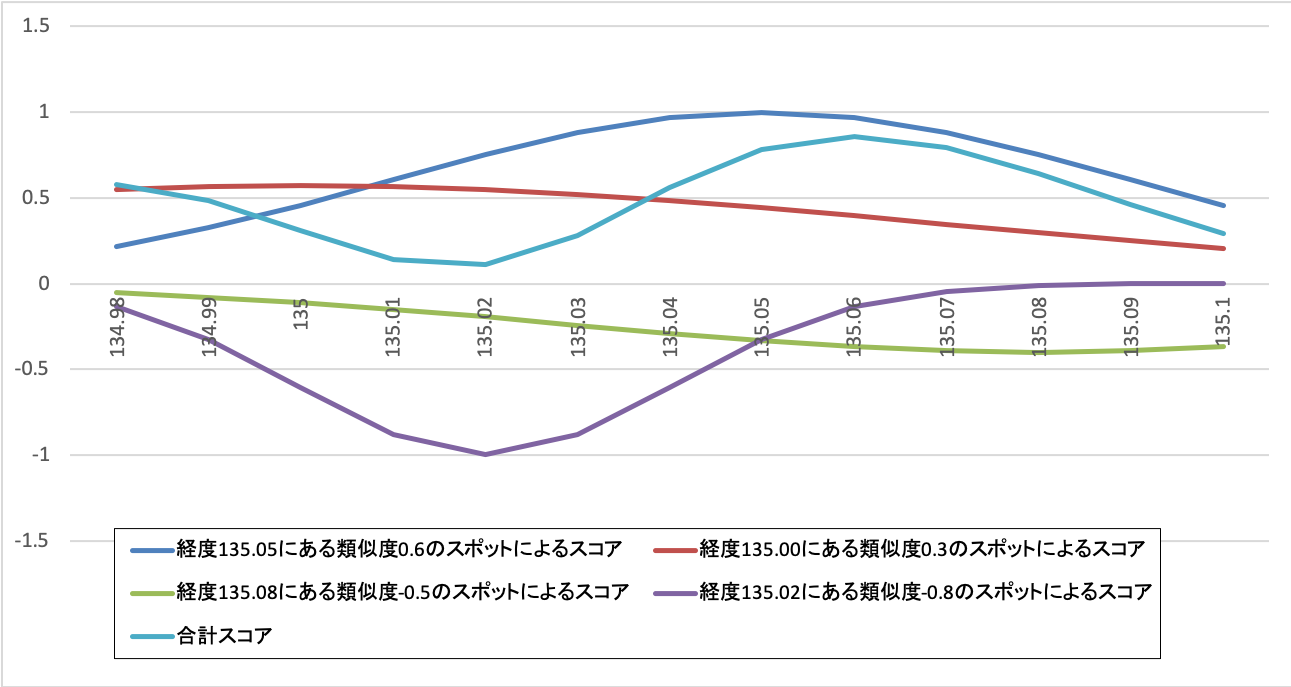
\includegraphics[clip,width=7.5cm]{picture/score_image2.png}
    \caption{既訪問スポットの経度座標計算の例}
    \label{fig:image}
   \end{center}
\end{figure}

%%%%%%%%%%%%%%%%%%%%%%%%%%%%%%%%%%%%%%%%%%
%%%%%%%%%%%%%%%%%%%%%%%%%%%%%%%%%%%%%%%%%%
\section{対応関係の可視化の評価}
\label{sec:対応関係の可視化評価}
%%%%%%%%%%%%%%%%%%%%%%%%%%%%%%%%%%%%%%%%%%
\subsection{実験内容}
未訪問スポットの説明性向上のための観光スポットの対応関係可視化手法の評価を行うため,以下の3つの提示手法を使って比較する.
図\ref{fig:P},図\ref{fig:L},図\ref{fig:T}は3つの提示手法それぞれのプロトタイプシステムとなっている.
黒いピンは入力した既訪問スポット,赤いピンは未訪問エリア内のスポットを意味している.
表示が重なることもあるため,黒いピンをクリックすると既訪問スポット名を吹き出しでも表示する.
また,3つの提示手法において,類似度が「0.0」以下であれば,関係を表現するキーワードが「なし」と表示する.
これは負の関係を表すキーワードは一般的に理解しにくいためである.
\begin{figure*}[t]
  \begin{center}
    \begin{tabular}{c}

      \begin{minipage}{0.33\hsize}
        \begin{center}
          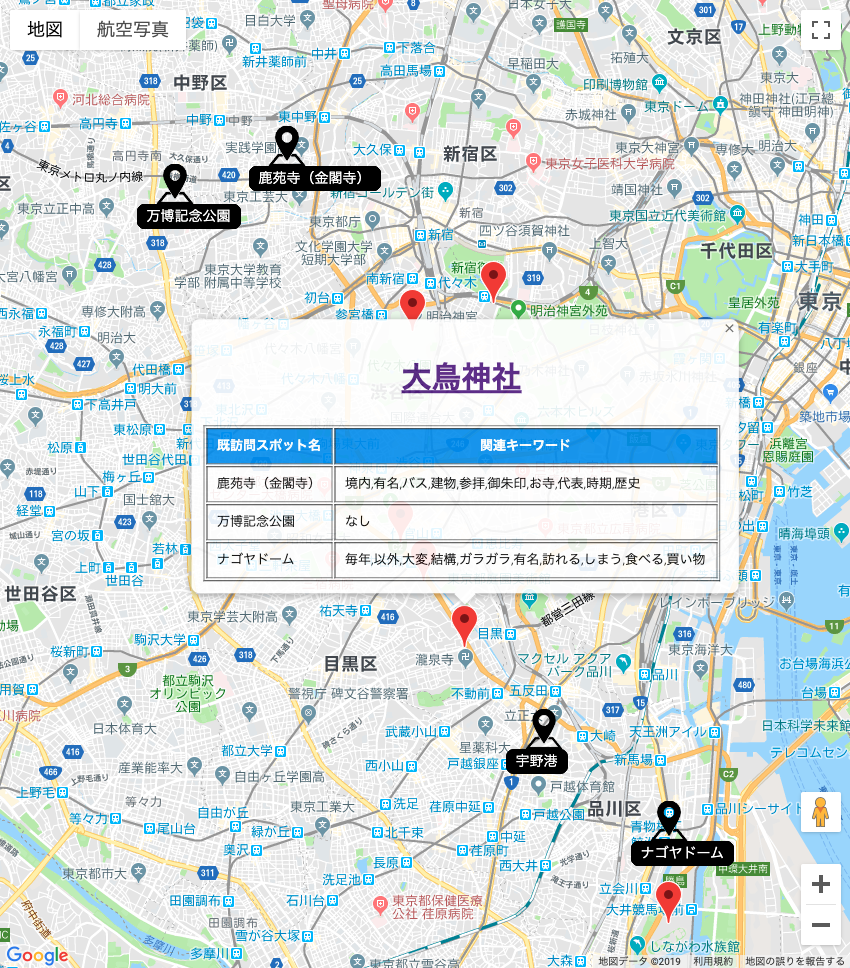
\includegraphics[clip, width=5cm]{picture/position_map2.png}
          \hspace{0.1cm}
          \caption{位置関係($Position\_Map$)}
          \label{fig:P}
        \end{center}
      \end{minipage}

      \begin{minipage}{0.33\hsize}
        \begin{center}
          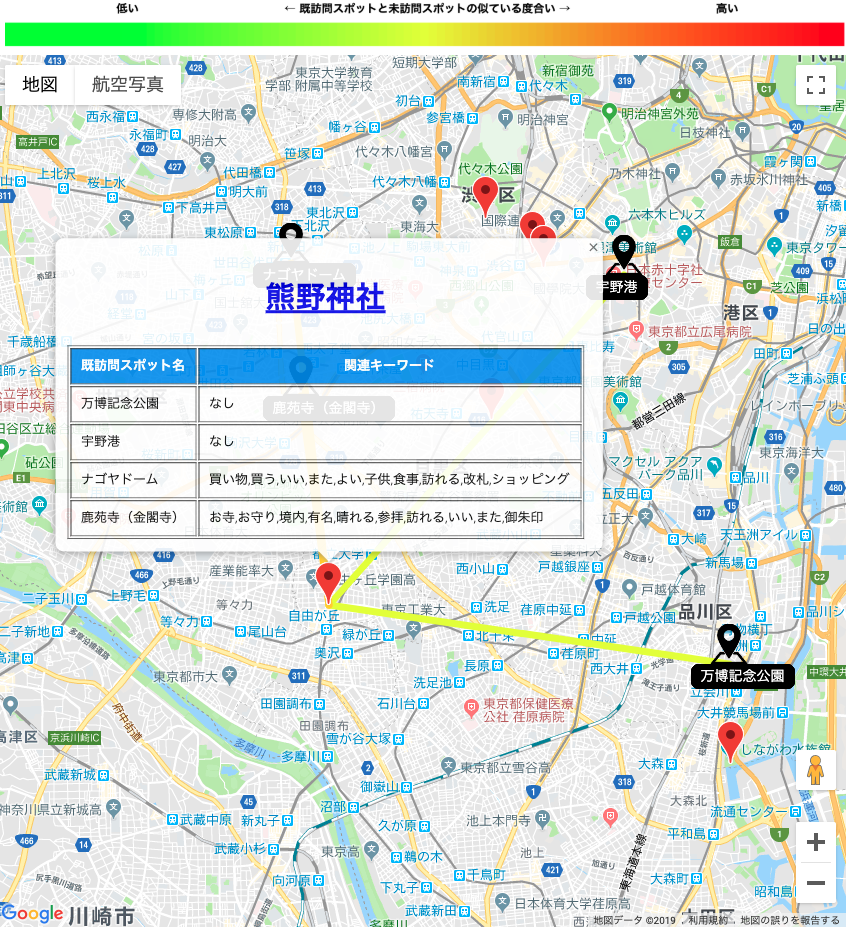
\includegraphics[clip, width=5.1cm]{picture/line_map2.png}
          \hspace{0.1cm}
          \caption{位置関係+線($Line\_Map$)}
          \label{fig:L}
        \end{center}
      \end{minipage}

      \begin{minipage}{0.33\hsize}
        \begin{center}
          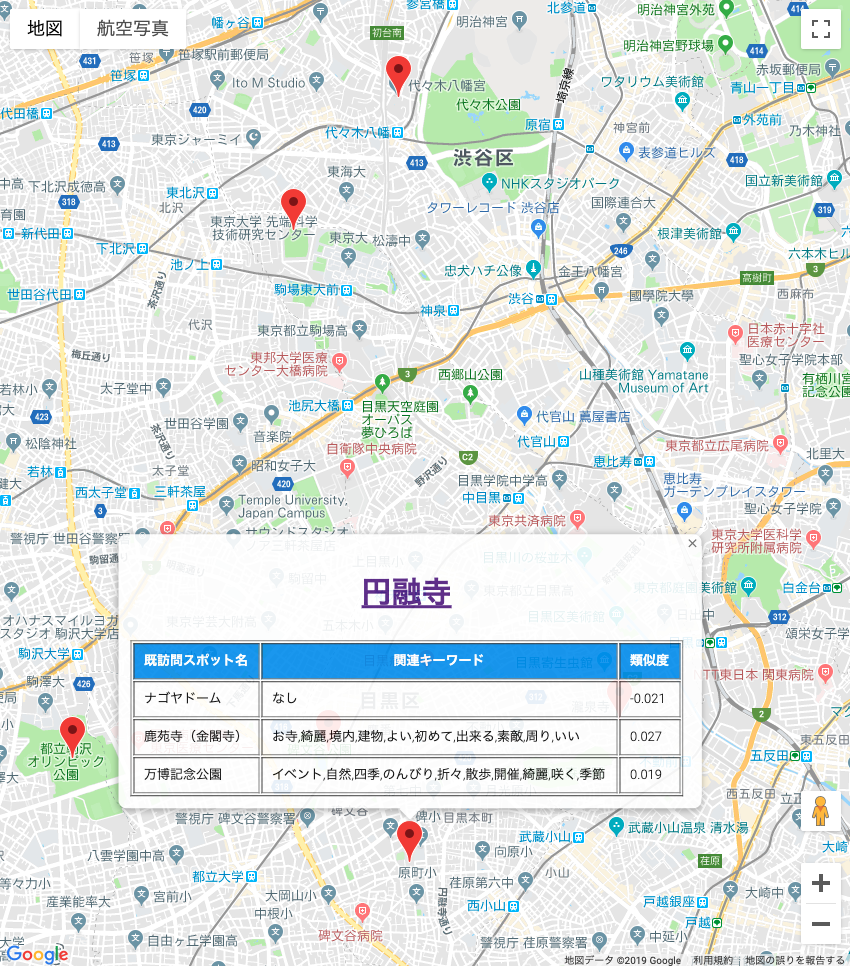
\includegraphics[clip, width=5cm]{picture/table_map2.png}
          \hspace{0.1cm}
        \caption{表形式($Table\_Map$)}
        \label{fig:T}
        \end{center}
      \end{minipage}

    \end{tabular}
  \end{center}
\end{figure*}

$Position\_Map$(図\ref{fig:P})では,検索対象のスポットと既訪問スポットの関連度を全体的な位置関係で表現している.
既訪問スポットは実際の座標ではなく,提案手法で決定した座標で表示される.
赤いピンをクリックすると詳細情報が表示される.
詳細情報は,未訪問スポット名,対応する既訪問スポット名,未訪問スポットと既訪問スポットの関係を表現するキーワードである.

$Line\_Map$(図\ref{fig:L})では,位置関係による提示に加えて線の色を使って表現している.
線の色は赤いピンと黒いピンの類似度を示している.
線は緑色に近いと類似度が低く,赤色に近いと類似度が高いことを意味している.
赤いピンをクリックすると詳細情報が表示される.
詳細情報は,$Position\_Map$と同じく,未訪問スポット名,対応する既訪問スポット名,未訪問スポットと既訪問スポットの関係を表現するキーワードである.

$Table\_Map$(図\ref{fig:T})では,位置関係や線は用いずに,$Line\_Map$で表現していたすべての情報を表形式でまとめて表現している.
詳細情報は,現在選択している未訪問スポット名と,対応する既訪問スポット名,未訪問スポットと既訪問スポットの関係を表現するキーワード,類似度である.
類似度の値は「-1.0から1.0」の間になる.
「-1.0」はもっとも類似せず,「1.0」はもっとも類似することを意味している.

%%%%%%%%%%%%%%%%%%%%%%%%%%%%%%%%%%%%%%%%%%
\subsection{実験手順}
クラウドソーシングのサービスである,CrowdWorks\footnote{https://crowdworks.jp}を利用して75人合計120件のデータを集めた.
まず,被験者は3個から9個の自分が既に訪れたことのある,かつ気に入った観光スポットを入力した.
次に,被験者は旅行などで行ったことがなく,これから訪れたい都道府県やエリアを入力した.

本実験では,各提示手法において,検索スポットが重複しないように振り分け,3つの提示手法を連続して利用した.
それぞれの提示手法において,被験者は検索スポットから行き先を決定した.
このとき,表示順に影響をなくすために,6パターンの表示順を作成し,被験者はランダムに1つの表示順で実験を行う.
実験を行った後,以下の項目について評価する.
\begin{itemize}
  \item 各提示手法の行き先の決定しやすさ
  \item $Position\_Map$と$Line\_Map$どちらのほうが,訪問履歴との関係がわかりやすかったか
  \item $Line\_Map$と$Table\_Map$どちらのほうが,訪問履歴との関係がわかりやすかったか
  \item 各提示手法の訪問先決定までにかかった体感時間
  \item 各提示手法の訪問先決定までにかかった労力
\end{itemize}
また,それぞれの手法について,自由記述で意見を書いてもらった.

%%%%%%%%%%%%%%%%%%%%%%%%%%%%%%%%%%%%%%%%%%
\subsection{実験結果と考察}
\begin{table}[t]
    \caption{行き先の決定しやすさの回答数割合}
    \label{table:行き先の決定しやすさ}
    \centering
    \begin{tabular}{l|rrrrr|l}
    \hline
    決定しやすさ   & \multicolumn{1}{l}{1} & \multicolumn{1}{l}{2} & \multicolumn{1}{l}{3} & \multicolumn{1}{l}{4} & \multicolumn{1}{l|}{5} & 平均    \\ \hline
    $Position\_Map$ & 5.0\%                & 15.8\%               & 15.0\%               & 51.7\%               & 12.5\%                & 3.51 \\
    $Line\_Map$     & 2.5\%                & 12.5\%               & 19.2\%               & 50.0\%               & 15.8\%                & 3.64 \\
    $Table\_Map$    & 3.3\%                & 5.8\%                & 35.0\%               & 46.7\%               & 9.2\%                 & 3.53 \\ \hline
    \end{tabular}
\end{table}
表\ref{table:行き先の決定しやすさ}は3つの提示手法それぞれの行き先の決定しやすさを5段階評価した回答数である.
5はとても決定しやすい,1はとても決定しづらいを意味している.
表\ref{table:行き先の決定しやすさ}の平均値から$Line\_Map$がもっとも決定しやすいことがわかった.
$Line\_Map$は$Position\_Map$より決定しやすい理由として,$Line\_Map$は位置情報提示に加えて,線を描くことによって,より既訪問スポットと未訪問スポットの対応関係を表現することができたためと考えられる.
ただし,3つの提示手法について$t$検定を行った結果,それぞれ有意差があるとはいえなかった.

\begin{table}[t]
    \caption{$Position\_Map$と$Line\_Map$の訪問履歴との関係の回答数割合}
    \label{table:PLの訪問履歴との関係}
    \centering
    \begin{tabular}{l|r}
    \hline
    回答    & 回答数の割合 \\
    \hline
    $Position\_Map$がわかりやすかった   & 15.8\% \\
    $Position\_Map$がややわかりやすかった & 28.3\% \\
    どちらでもない                  & 20.0\% \\
    $Line\_Map$がややわかりやすかった     & 24.2\% \\
    $Line\_Map$がわかりやすかった       & 11.7\% \\ \hline
    \end{tabular}
\end{table}
\begin{table}[t]
    \caption{$Line\_Map$と$Table\_Map$の訪問履歴との関係の回答数割合}
    \label{table:LTの訪問履歴との関係}
    \centering
    \begin{tabular}{l|r}
    \hline
    回答    & 回答数の割合 \\
    \hline
    $Line\_Map$がわかりやすかった    & 12.5\% \\
    $Line\_Map$がややわかりやすかった  & 28.3\% \\
    どちらでもない               & 27.5\% \\
    $Table\_Map$がややわかりやすかった & 24.2\% \\
    $Table\_Map$がわかりやすかった   & 7.5\%  \\ \hline
    \end{tabular}
\end{table}
表\ref{table:PLの訪問履歴との関係}は$Position\_Map$と$Table\_Map$どちらのほうが,訪問履歴との関係がわかりやすかったかの回答数の割合となっている.
表\ref{table:PLの訪問履歴との関係}から$Position\_Map$がわかりやすいの割合が$44.2\%$に対して,$Line\_Map$が$35.8\%$のため,$Position\_Map$のほうがわかりやすいといえる.
一方,表\ref{table:行き先の決定しやすさ}では,$Position\_Map$がもっとも決定しづらいといえる.
理由として,$Position\_Map$は他の2つの提示手法と比べると,決定しづらい回答数が多くなっている.
また,「黒いピンと赤いピンの類似距離という関係性があまりよくわかりません」といった意見の被験者が多数おり,強く好まない被験者が一定数が存在するため,このような結果となったと考える.
位置関係を表現する際に,仮想的な地物の類似性を視覚的に表していることが明確にわかるインタフェースにする必要がある.
また,表\ref{table:LTの訪問履歴との関係}は$Line\_Map$と$Table\_Map$の訪問履歴との関係のわかりやすさの回答数の割合となっている.
表\ref{table:LTの訪問履歴との関係}から$Line\_Map$がわかりやすいの割合が$40.4\%$に対して,$Table\_Map$が$31.7\%$のため,$Line\_Map$のほうがわかりやすい.

\begin{table}[t]
    \caption{$Position\_Map$と$Line\_Map$の決定しやすさと関係わかりやすさについての回答数}
    \label{table:決定しやすさと関係わかりやすさについての回答数}
    \centering
    \begin{tabular}{l|l|r}
    \hline
    決定のしやすさ     & 関係のわかりやすさ      & \multicolumn{1}{l}{回答数} \\ \hline
    $P$は$L$よりしやすい & $P$が$L$よりわかりやすい & 18                       \\
    $L$は$P$よりしやすい & $P$が$L$よりわかりやすい & 3                        \\
    $P$は$L$よりしやすい & $L$が$P$よりわかりやすい & 1                        \\
    $L$は$P$よりしやすい & $L$が$P$よりわかりやすい & 23                       \\ \hline
    \end{tabular}
\end{table}
表\ref{table:決定しやすさと関係わかりやすさについての回答数}は同一の被験者の表\ref{table:行き先の決定しやすさ}と表\ref{table:PLの訪問履歴との関係}の結果を比較し,$Position\_Map$と$Line\_Map$の行き先の決定しやすさと訪問履歴との関係のわかりやすさについての回答数となっている.
表\ref{table:行き先の決定しやすさ}に関しては,どちらに大きな値をつけたかを集計している.
行き先決定のしやすさと訪問履歴の互いの影響に関して,決定しやすさと訪問履歴の評価が一致で回答した数はが異なると回答した数より多いため,互いに影響があることが考えられる.
% また,行き先決定のしやすさに関してて$Line\_Map$のほうが決定しやすいと回答する数が多い.
% 訪問履歴との関係に関して$Position\_Map$のほうが関係がわかりやいと回答する数が多い.

\begin{table}[t]
    \caption{訪問先決定までにかかった体感時間の回答数割合}
    \label{table:訪問先決定までにかかった体感時間}
    \centering
    \begin{tabular}{l|rrrrr|r}
    \hline
                  & \multicolumn{1}{l}{1} & \multicolumn{1}{l}{2} & \multicolumn{1}{l}{3} & \multicolumn{1}{l}{4} & \multicolumn{1}{l|}{5} & \multicolumn{1}{l}{平均} \\ \hline
    $Position\_Map$ & 10.0\%               & 40.8\%               & 30.0\%               & 15.8\%               & 3.3\%                & 2.62                   \\
    $Line\_Map$     & 13.3\%               & 35.8\%               & 30.0\%               & 15.8\%               & 5.0\%                & 2.63                   \\
    $Table\_Map$    & 9.2\%                & 33.3\%               & 35.8\%               & 18.3\%               & 3.3\%                & 2.73                   \\ \hline
    \end{tabular}
\end{table}

\begin{table}[t]
    \caption{訪問先決定までにかかった労力の回答数割合}
    \label{table:訪問先決定までにかかった労力}
    \centering
    \begin{tabular}{l|rrrrr|r}
    \hline
                  & \multicolumn{1}{l}{1} & \multicolumn{1}{l}{2} & \multicolumn{1}{l}{3} & \multicolumn{1}{l}{4} & \multicolumn{1}{l|}{5} & \multicolumn{1}{l}{平均} \\ \hline
    $Position\_Map$ & 14.2\%               & 35.8\%               & 27.5\%               & 16.7\%               & 5.8\%                 & 2.64                   \\
    $Line\_Map$     & 15.8\%               & 36.7\%               & 30.0\%               & 12.5\%               & 5.0\%                 & 2.54                   \\
    $Table\_Map$    & 11.7\%               & 33.3\%               & 34.2\%               & 15.8\%               & 5.0\%                 & 2.69                   \\ \hline
    \end{tabular}
\end{table}

表\ref{table:訪問先決定までにかかった体感時間}は3つ提示手法それぞれの訪問先を決定するまでにかかった体感時間を5段階評価した回答数である.
1は訪問先決定するまでに短い時間で,5は長い時間で決定していることを意味している.
表\ref{table:訪問先決定までにかかった労力}は3つ提示手法それぞれの訪問先決定するまでにかかった労力を5段階評価した回答数である.
1は訪問先決定するまで少ない労力で,5は多い労力で決定していることを意味している.
体感時間と労力の相関係数を計算すると$0.74$と強い正の相関があり,体感時間が短いと労力も少なく,体感時間が長いと労力も多くなる.
% 表\ref{table:訪問先決定までにかかった体感時間}と表\ref{table:訪問先決定までにかかった労力}から$Table\_Map$がもっとも被験者にとって手間がかかっていることがわかる.
訪問先決定までにかかった体感時間が短いと回答した数の割合は$Position\_Map$が$50.8\%$,$Line\_Map$が$49.2\%$,$Table\_Map$が$42.5\%$となっている.
よって,$Position\_Map$がかかった体感時間がもっとも短く,$Table\_Map$がもっとも長いことがわかった.
訪問先決定までにかかった労力が少ないと回答した数の割合は$Position\_Map$が$50.0\%$,$Line\_Map$が$52.5\%$,$Table\_Map$が$45.0\%$となっている.
よって,$Line\_Map$がかかった労力がもっとも少ない,$Table\_Map$がもっとも多いことがわかった.
以上から,$Line\_Map$は体感時間が短くかつ労力も少なく訪問先を決定することができ,$Table\_Map$はもっとも被験者にとって手間がかかっていることがわかった.
対応関係を位置情報で表すことによって,表形式の時間と労力の問題点について改善することができるといえる.
$Line\_Map$は被験者に提示する文字の情報を少なくして,線の色と位置関係を使って既訪問スポットと未訪問スポット対応関係を見せることによって,他の2つの提示手法と比べると理解容易化することができたと考えられる.


%%%%%%%%%%%%%%%%%%%%%%%%%%%%%%%%%%%%%%%%%%
%%%%%%%%%%%%%%%%%%%%%%%%%%%%%%%%%%%%%%%%%%
\section{まとめと今後の課題}
\label{sec:まとめと今後の課題}

本研究では,ユーザが行きたい観光スポットが決まっていない場合に,ユーザの事前知識が不足しているため,観光検索サイトを使用してランキング,おすすめ情報やカテゴリなどを基に検索された観光スポットに対する理解が困難であることに着目した.
また,関連付けした未訪問スポットと既訪問スポットの関連性をよりユーザの理解容易化するために,地図上に既訪問スポットと未訪問スポットの対応関係を可視化する手法を提案し,3種類の可視化インタフェースを作成し,比較実験を行った.

$Table\_Map$に関して,類似度を数値のままに表形式で被験者に提示しているため,被験者は訪問先を決定するには時間と労力をついやす必要がある.
よって,表示位置で関係を表す$Position\_Map$と$Line\_Map$より決定しづらいことを確認した.
$Position\_Map$に関して類似度を使って計算した結果を既訪問スポットの位置情報のみ被験者に提示しているため,既訪問スポットと未訪問スポットとの関連性を勘違いする人がいることがわかった.
これは,$Line\_Map$でも潜在的に持つ問題であり,誤解を与えない表現を検討する必要がある.

今後の課題としては,文字をユーザに提示することによって行き先の決定に時間と労力をかかるため,既訪問スポットと対象観光スポットの関係を表現するためにキーワード以外の情報を使ってユーザに提示する予定である.

%%%%%%%%%%%%%%%%%%%%%%%%%%%%%%%%%%%%%%%%%%
\section*{謝辞}
%%%%%%%%%%%%%%%%%%%%%%%%%%%%%%%%%%%%%%%%%%
本研究の一部は,2019年度科研費基盤研究(C)(課題番号:18K11551)によるものです.ここに記して謝意を表すものとします.

%%%%%%%%%%%%%%%%%%%%%%%%%%%%%%%%%%%%%%%%%%
% 文献 Reference
%%%%%%%%%%%%%%%%%%%%%%%%%%%%%%%%%%%%%%%%%%
\vspace{2em}

% \bibliographystyle{junsrt}
% \bibliography{man}

%%%%%%%%%%%%%%%%%%%%%%%%%%%%%%%%%%%%%%%%%%
\begin{thebibliography}{10}
  \bibitem{潘}
    潘 健太, 北山 大輔:
      ユーザの既訪問スポットの位置付けに基づく未訪問スポットの説明手法,
      第11回データ工学と情報マネジメントに関するフォーラム(DEIM Forum 2019), H7-2, 2019
 \bibitem{櫻川2015}
    櫻川 直洋, 廣田 雅春, 石川 博, 横山 昌平:
      ジオタグ付き写真の撮影者を在住者と観光者に分類することによるホットスポットの発見,
      第7回データ工学と情報マネジメントに関するフォーラム(DEIM Forum 2015), F6-3, 2015
  \bibitem{櫻川2016}
    櫻川 直洋, 廣田 雅春, 石川 博, 横山 昌平:
      ジオタグ付き写真を用いたイベントとその穴場スポットの発見,
      第8回データ工学と情報マネジメントに関するフォーラム(DEIM Forum 2016), H5-3, 2016
 \bibitem{倉田}
    倉田 陽平, 杉本 興運, 矢部 直人:
      あえて案内しない着地型観光案内ー観光関心点群の抽出と活用,
      第19回地理情報システム学会講演論文集, 2010
  \bibitem{Kitamura}
    Kitamura, R. and Itoh, T.:
      Tourist Spot Recommendation Applying Generic Object Recognition with Travel Photos,
      In 2018 22nd International Conference Information Visualisation, pp.1-5, 2018
 \bibitem{上村}
    上村 幸汰, 桂井 麻里衣, 真木 勇人, 後藤 亮介:
      タグ付き画像を用いたファッションスタイルの関係性の可視化,
      第11回データ工学と情報マネジメントに関するフォーラム(DEIM Forum 2019), E8-2, 2019
\end{thebibliography}

\end{document}
